\chapter{Project defence}
\label{ch:project_defence}

In what follows a high-level discussion is held on the created code.
The \texttt{README.md} file contains a more informal discussion on the functionality as well.
Multiple figures and screenshots were made to illustrate the different parts of the project.
Some of these figures are provided in the extra figures list at the end of this report.
For more technical details the reader is invited to read the documentation and comments in the code.


%------------------------------------

\section{Used patterns}
\label{sec:main_patterns}

The main used patterns are: \texttt{Forward Flow}, \texttt{Aggregator} and \texttt{Domain Object}.
A custom \texttt{Pr\-ority Queue Mailbox} was implemented as well.
The \texttt{Domain Object} pattern makes for a clear separation of business logic and communication logic as requested by the assignment.
A type of \texttt{Aggregator} pattern is used to collect all requested items of a purchase.
The \texttt{Forward Flow} pattern is not so much of a pattern as it is a \textit{mind set}.
Special care was taken to eliminate non-necessary \textit{man in the middle} by specifying \texttt{replyTo} addresses.
The custom \texttt{priority queue mailbox} that is used as default \texttt{Mailbox} for all \texttt{Actors} gives a higher priority to messages from \texttt{Prime} members.


%------------------------------------

\section{Managing stock houses}
\label{sec:managing_stock}

Whilst not specified in the assignment, it is possible to add stock houses and inventory through messages such as \texttt{AddStockHouse} and \texttt{AddProductToStockHouse}.
Adding \texttt{StockHouse} objects is done in business logic, inside a \texttt{StockHouseManager}.
This manager will keep a list of stock houses it created.
The \texttt{StockHouseManagerService}, responsible for the communication logic, also stores the \texttt{ActorRef} and \texttt{Name} for each of the added stock house.
It does this by maintaining a list of \texttt{NamedActor} objects, which have a unique name based on the stock house address and the Actor's \texttt{ActorRef}.
The clear separation of business logic is noticeable here and everywhere in the project, as the \texttt{Domain Object} pattern is used.
The \texttt{Main} loop initialises some stock houses and inventory, as displayed in figure \ref{fig:managing_stockhouse}


%------------------------------------

\section{Starting a purchase process and ephemeral children}
\label{sec:start_process}

\begin{figure}[H]
    \centering
    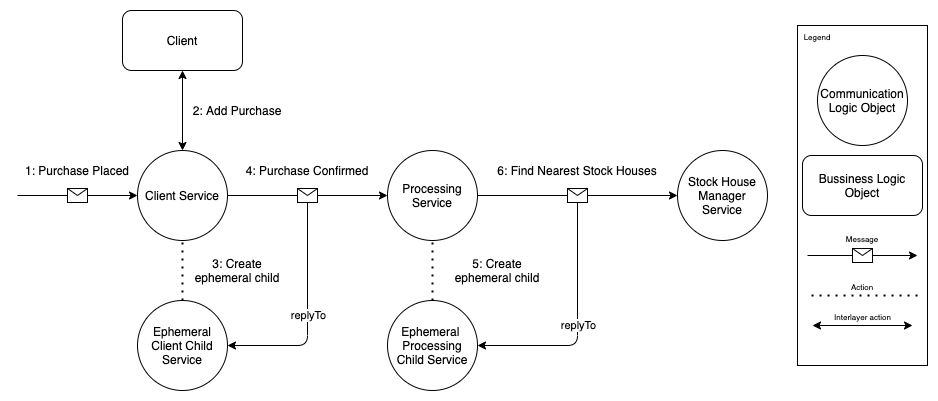
\includegraphics[width=0.9\linewidth]{images/initial_phase.png}
    \captionsetup{width=0.75\linewidth}
    \captionsetup{justification=centering}
    \caption{Simplified representation of first phase of purchase process.}
    \label{fig:first-phase}
\end{figure}

The first phase of the purchase process is shown in figure \ref{fig:first-phase}.
To start the process, the \texttt{ClientService}, from the \texttt{client} who placed the purchase, should receive a \texttt{PurchasePlaced} message.
This will first, in the \textit{domain logic} object of class \texttt{Client}, update the purchases list. 
It will then in \textit{communication logic} create an ephemeral \texttt{ClientChildService} responsible for further processing this purchase.
It then sends out a \texttt{Purchase\-Confirmed} message to the \texttt{ProcessingService}.
It is noted here that the \texttt{Forward Flow} pattern is in place by supplying the \texttt{replyTo} address of the ephemeral child.
It is also noted here that, as is the case for more messages in this project, a prime alternative message \texttt{PurchaseConfirmedPrime} can also be sent out depending on if the requesting client is a prime member.
Why a different message is used for \texttt{Prime} members will become clear when discussing the priority mailbox.

Once the \texttt{ProcessingService} receives a \texttt{PurchaseConfirmed} message, it also will create an ephemeral \texttt{ProcessingChildService} responsible for further handling this purchase.
It will also message the \texttt{StockHouseManagerService} a \texttt{FindNearestStockHouses} request (prime alternative available).
This request also contains the \texttt{replyTo} address for the just created ephemeral child, keeping in mind the \texttt{Forward Flow} pattern.

%------------------------------------

\section{Aggregating items to fulfill purchases}
\label{sec:finishing_process}

\begin{figure}[H]
    \centering
    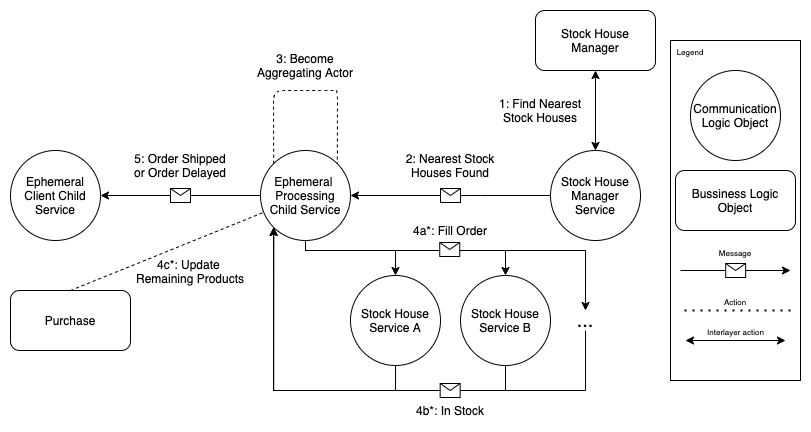
\includegraphics[width=0.8\linewidth]{images/aggr_phase.png}
    \captionsetup{width=0.9\linewidth}
    \captionsetup{justification=centering}
    \caption{Simplified representation of aggregating phase of purchase process.}
    \label{fig:aggr-phase}
\end{figure}

The aggregating phase of the purchase process is shown in figure \ref{fig:aggr-phase}.
Once the nearest stock houses are found in \textit{business logic}, the ephemeral \texttt{Processing\-Child\-Service} receives a \texttt{Nearest\-Stock\-Houses\-Found} message.
Upon receiving this message, the ephemeral child will change its behaviour by becoming an aggregating actor.
This aggregating happens by sending out \texttt{FillOrder} messages (prime alternative available) to the found nearest stock houses until either:
\begin{itemize}
    \item All items of the purchase are received through \texttt{InStock} messages. The ephemeral client child will receive a \texttt{OrderShipped} message.
    \item There are no stock houses to contact left and the order is not yet complete. The ephemeral client child will receive a \texttt{OrderDelayed} message.
\end{itemize}
It is noted that the sending out of the \texttt{FillOrder} messages happens incrementally rather than all at once.
The latter is often the aggregator pattern approach but for simplification reasons, the incremental variant seemed fit.
Some screenshots of this process are shown in figure \ref{fig:purchase_process}.

%------------------------------------

\section{Handling prime membership}
\label{sec:prime}

Handling the requests of prime members with priority is done by using a custom made priority mailbox\footnote{\url{https://doc.akka.io/docs/akka/current/mailboxes.html}}: \texttt{PrimePriorityMailbox}.
This mailbox simply ensures prime messages have a higher priority than other messages.
It's noted that only messages which can be in an inbox with both prime and non-prime member messages require special attention.
Indeed, prioritizing \texttt{InStock} messages, and others, for prime members has no benefit. They are sent to an ephemeral child of the \texttt{ClientService} which only receives messages for one \texttt{Client} and thus only prime or non-prime messages.
Figure \ref{fig:mailbox_implement} shows the implementation of this mailbox.